%% LyX 1.6.7 created this file.  For more info, see http://www.lyx.org/.
%% Do not edit unless you really know what you are doing.
\documentclass[english]{article}
\usepackage{amsmath}
\usepackage[T1]{fontenc}
\usepackage[latin9]{inputenc}
\usepackage{graphicx}
\usepackage{esint}
\usepackage{babel}
\usepackage{parskip}            % for \smallskip, \medskip and \bigskip

\begin{document}

\title{Pulse function}

\maketitle
$y(x)=\dfrac{1}{x}$

$\int_{o}^{\infty}dx$

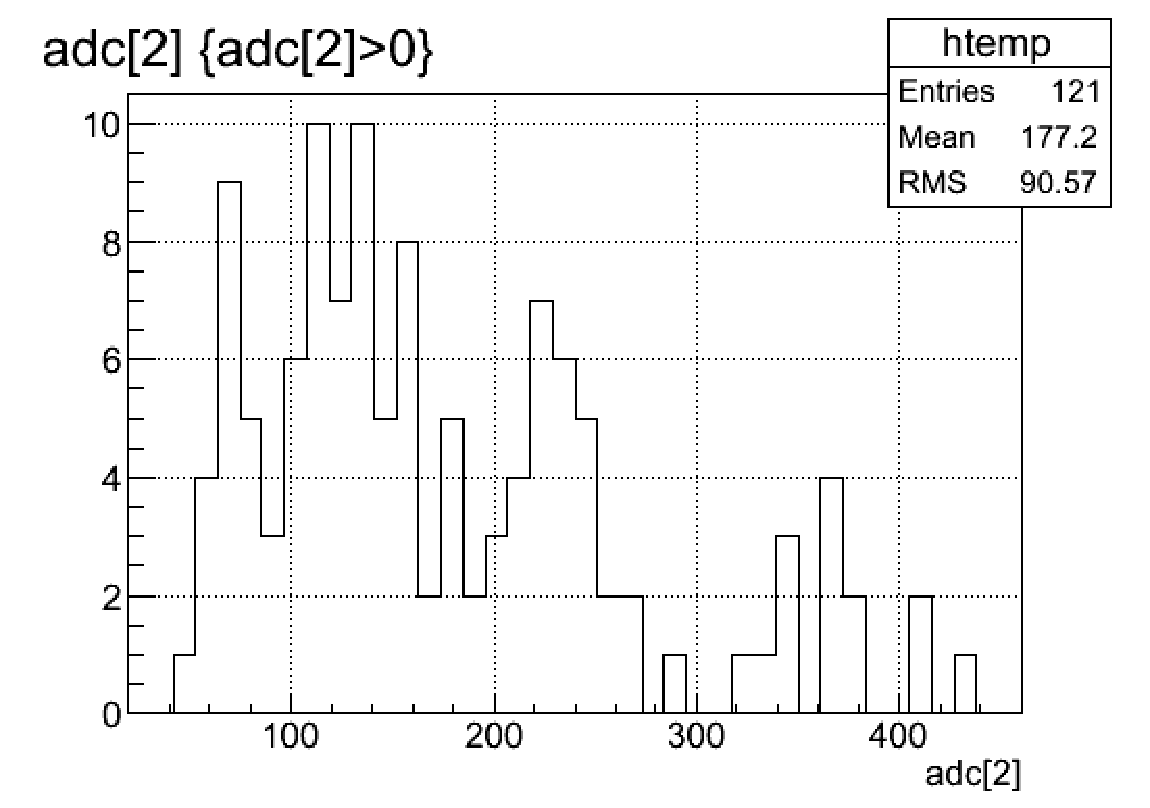
\includegraphics[scale=0.5]{/srv/zatserkl/work/psec/drs4/note/Na22_stm1}

channel 3

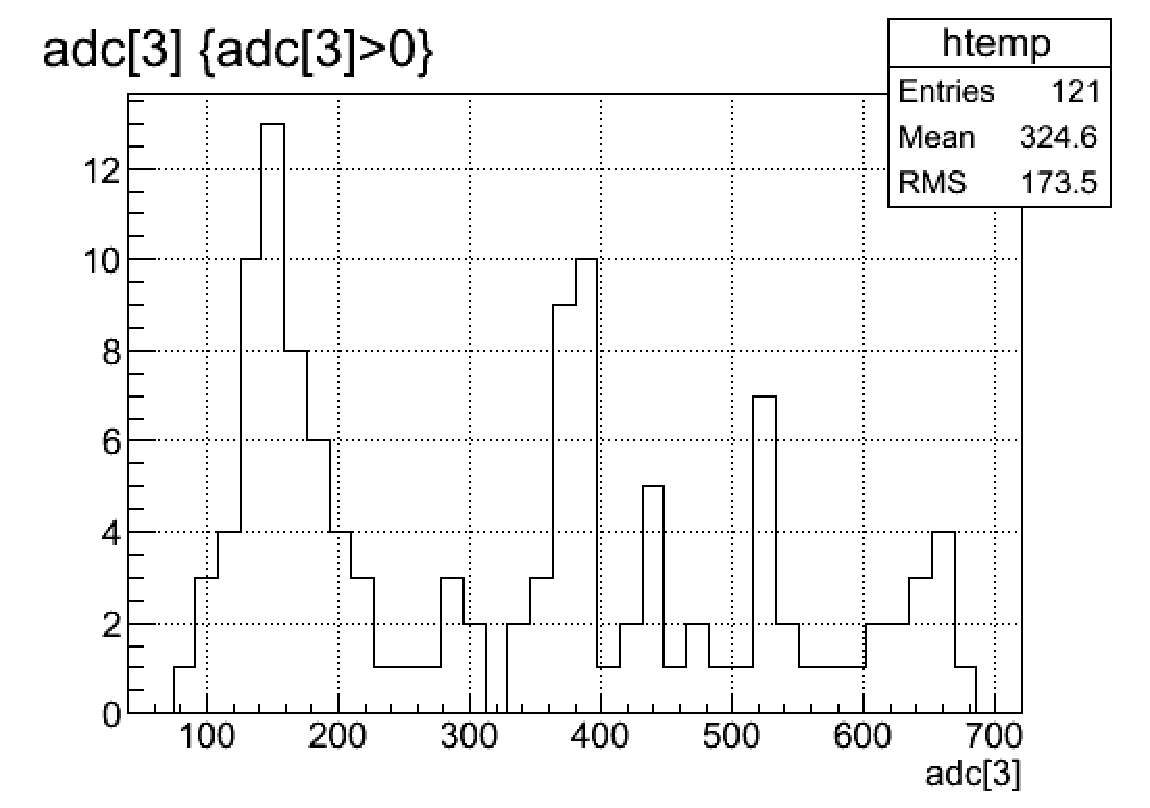
\includegraphics[scale=0.5]{/srv/zatserkl/work/psec/drs4/note/Na22_stm2}


\section{Derive the function}

Define the function as a charging/discharging of capacitor:

$p(t)=(1-e^{-t/\tau})e^{-t/\tau}$, $t>0$

Smear this function by convolution with Gaussian with sigma $\sigma$.

$y(x)=\frac{1}{\sqrt{2\pi}\sigma}\int_{-\infty}^{\infty}p(t)e^{-\frac{(t-x)^{2}}{2\sigma^{2}}}dt$

because $p(t)=0$ for $t<0$

$y(x)=\frac{1}{\sqrt{2\pi}\sigma}\int_{0}^{\infty}p(t)e^{-\frac{(t-x)^{2}}{2\sigma^{2}}}dt$

or

$y(x)=\frac{1}{\sqrt{2\pi}\sigma}\int_{0}^{\infty}(1-e^{-t/\tau)})e^{-t/\tau}e^{-\frac{(t-x)^{2}}{2\sigma^{2}}}dt$

$y(x)=\frac{1}{\sqrt{2\pi}\sigma}\left[\int_{0}^{\infty}e^{-t/\tau}e^{-\frac{(t-x)^{2}}{2\sigma^{2}}}dt-\int_{0}^{\infty}e^{-t/\tau}e^{-\frac{(t-x)^{2}}{2\sigma^{2}}}dt\right]$

Denote 

$y(x)=\frac{1}{\sqrt{2\pi}\sigma}(I(x,\tau)-I(x,\tau/2))$

where 

$I(x,\tau)=I=\int_{0}^{\infty}e^{-t/\tau}e^{-\frac{(t-x)^{2}}{2\sigma^{2}}}dt$

Rewriting and expressing the complete square we will have

$I=\sigma\sqrt{2}e^{-(\frac{x}{\tau}-\frac{\sigma^{2}}{2\tau^{2}})}\int_{0}^{\infty}\frac{dt}{\sigma\sqrt{2}}e^{-(\frac{t}{\sigma\sqrt{2}}-\frac{1}{\sigma\sqrt{2}}(x-\frac{\sigma^{2}}{\tau}))^{2}}$

$=\sigma\sqrt{2}e^{-(\frac{x}{\tau}-\frac{\sigma^{2}}{2\tau^{2}})}\int_{-\frac{1}{\sigma\sqrt{2}}(x-\frac{\sigma^{2}}{\tau})}^{\infty}e^{-z^{2}}dz$ 

$=\sigma\sqrt{2}e^{-(\frac{x}{\tau}-\frac{\sigma^{2}}{2\tau^{2}})}(\int_{0}^{\frac{1}{\sigma\sqrt{2}}(x-\frac{\sigma^{2}}{\tau})}e^{-z^{2}}dz+\int_{0}^{\infty}e^{-z^{2}}dz)$

$=\sigma\sqrt{2}e^{-(\frac{x}{\tau}-\frac{\sigma^{2}}{2\tau^{2}})}(\frac{\sqrt{\pi}}{2}\frac{2}{\sqrt{\pi}}\int_{0}^{\frac{1}{\sigma\sqrt{2}}(x-\frac{\sigma^{2}}{\tau})}e^{-z^{2}}dz+\frac{\sqrt{\pi}}{2})$

$=\sigma\sqrt{2}e^{-(\frac{x}{\tau}-\frac{\sigma^{2}}{2\tau^{2}})}\frac{\sqrt{\pi}}{2}(1+\frac{2}{\sqrt{\pi}}\int_{0}^{\frac{1}{\sigma\sqrt{2}}(x-\frac{\sigma^{2}}{\tau})}e^{-z^{2}}dz)$

$=\sqrt{\frac{\pi}{2}}\sigma e^{-(\frac{x}{\tau}-\frac{\sigma^{2}}{2\tau^{2}})}(1+erf\frac{x-\frac{\sigma^{2}}{\tau}}{\sigma\sqrt{2}})$ 

$=\sqrt{\frac{\pi}{2}}\sigma e^{-(\frac{x}{\tau}-\frac{\sigma^{2}}{2\tau^{2}})}(1-erf\frac{\frac{\sigma^{2}}{\tau}-x}{\sigma\sqrt{2}})$

Finally,

$I(x,\tau)=\sqrt{\frac{\pi}{2}}\sigma e^{-(\frac{x}{\tau}-\frac{\sigma^{2}}{2\tau^{2}})}erfc\frac{\frac{\sigma^{2}}{\tau}-x}{\sigma\sqrt{2}}$

Correspondingly, 

$I(x,\tau/2)=\sqrt{\frac{\pi}{2}}\sigma e^{-(\frac{2x}{\tau}-\frac{2\sigma^{2}}{\tau^{2}})}erfc\frac{\frac{2\sigma^{2}}{\tau}-x}{\sigma\sqrt{2}}$

Now consider different value for rise and discharge time, $\tau_{1}$and
$\tau_{2}$.

Now

$p(x)=(1-e^{-\frac{t}{\tau_{1}}})e^{-\frac{t}{\tau_{2}}}$

and

$y(x)=\frac{1}{\sqrt{2\pi}\sigma}\int_{0}^{\infty}(1-e^{-t/\tau_{1})})e^{-t/\tau_{2}}e^{-\frac{(t-x)^{2}}{2\sigma^{2}}}dt$

$y(x)=\frac{1}{\sqrt{2\pi}\sigma}\left[\int_{0}^{\infty}e^{-t/\tau_{2}}e^{-\frac{(t-x)^{2}}{2\sigma^{2}}}dt-\int_{0}^{\infty}e^{-t(\frac{1}{\tau_{1}}+\frac{1}{\tau_{2}})}e^{-\frac{(t-x)^{2}}{2\sigma^{2}}}dt\right]$

Define $\tau_{12}=\frac{1}{\tau_{1}}+\frac{1}{\tau_{2}}$

Then

$y(x)=\frac{1}{\sqrt{2\pi}\sigma}\left[\int_{0}^{\infty}e^{-t/\tau_{2}}e^{-\frac{(t-x)^{2}}{2\sigma^{2}}}dt-\int_{0}^{\infty}e^{-\frac{t}{\tau_{12}}}e^{-\frac{(t-x)^{2}}{2\sigma^{2}}}dt\right]$

or

$y(x)=\frac{1}{\sqrt{2\pi}\sigma}(I(x,\tau_{2})-I(x,\tau_{12}))$

After some optimization

$y(x)=\frac{1}{\sqrt{2\pi}\sigma}\sqrt{\pi/2}\sigma[I'(x,\tau_{2})-I'(x,\tau_{12})]$

finally

$y(x)=\frac{1}{2}[I'(x,\tau_{2})-I'(x,\tau_{12})]$

where

$I'(x,\tau)=e^{-(\frac{x}{\tau}-\frac{\sigma^{2}}{2\tau^{2}})}erfc\frac{\frac{\sigma^{2}}{\tau}-x}{\sigma\sqrt{2}}$

Example.


\section{Convolution with scintillator decay}

Lets represent scintillator decay function as 

$s(t)=\frac{1}{T}e^{-t/T}$, $t\geq0$

Pulse function $p(t)=A(1-e^{-t/\tau_{1}})e^{-t/\tau_{2}}$

Convolution of the pulse function with scintillator decay.

Contribution to time moment $x$ from pulse originated in $t$ ($t\leq x$)
with weight $s(t)$.

$p(x-t)s(t)$

and 

$P(x)=\int_{0}^{x}p(x-t)s(t)dt$

$P(x)=\frac{A}{T}\int_{0}^{x}(1-e^{-\frac{x-t}{\tau_{1}}})e^{-\frac{x-t}{\tau_{2}}}e^{-t/T}dt$,
$x\geq t$

$=\frac{A}{T}(I_{1}^{T}-I_{2}^{T})$

where

$I_{1}^{T}=\int_{0}^{x}e^{-\frac{x-t}{\tau_{2}}}e^{-t/T}dt$

$I_{2}^{T}=\int_{0}^{x}e^{-(\frac{1}{\tau_{1}}+\frac{1}{\tau_{2}})(x-t)}e^{-t/T}dt$

Define 

$I^{T}(x,\tau,T)=\int_{0}^{x}e^{-x/\tau}e^{t/\tau}e^{-t/T}dt$

$=e^{-x/\tau}\int_{0}^{x}e^{(\frac{1}{\tau}-\frac{1}{T})t}dt$

$=e^{-x/\tau}\frac{1}{\frac{1}{\tau}-\frac{1}{T}}\int_{0}^{(\frac{1}{\tau}-\frac{1}{T})x}e^{z}dz$

$=e^{-x/\tau}\frac{1}{\frac{1}{\tau}-\frac{1}{T}}(e^{(\frac{1}{\tau}-\frac{1}{T})x}-1)$

Note, that $\frac{1}{\frac{1}{\tau}-\frac{1}{T}}(e^{(\frac{1}{\tau}-\frac{1}{T})x}-1)\rightarrow x$
as $\frac{1}{\tau}-\frac{1}{T}\rightarrow0$

Then, in terms of $I^{T}(x,\tau,T)$

$I_{1}^{T}=I^{T}(x,\tau_{2},T)$, NB: $\tau_{2}$

$I_{2}^{T}=I^{T}(x,\tau_{12},T)$, where $\tau_{12}=\frac{1}{\tau_{1}}+\frac{1}{\tau_{2}}$ 

The End.
\end{document}
